\documentclass[13pt,a4paper]{extarticle}
% =========================================================
% FONT CHU - TOAN BO BAO CAO DUNG TIMES NEW ROMAN
% =========================================================
\usepackage{fontspec}
% Ưu tiên Times New Roman; dùng font cùng họ Times nếu máy biên dịch chưa có TNR.
\IfFontExistsTF{Times New Roman}{%
    \setmainfont{Times New Roman}
    \setsansfont{Times New Roman}
    \setmonofont{Times New Roman}
}{%
    \setmainfont{TeX Gyre Termes}
    \setsansfont{TeX Gyre Termes}
    \setmonofont{TeX Gyre Termes}
}
% =========================================================
% THU VIEN
% =========================================================
\usepackage{geometry}
\usepackage{tikz}
\usetikzlibrary{
    arrows.meta,
    positioning,
    shapes.geometric,
    fit,
    calc
}
\usepackage{graphicx}
% Biên dịch tại ketqua/ hoặc từ thư mục package đều tìm được các ảnh có sẵn.
\graphicspath{{./}{ketqua/}{images/}}
\usepackage{array}
\usepackage{float}
\usepackage{tabularx}
\usepackage{booktabs}
\usepackage{amsmath}
\usepackage{fancyvrb}
\usepackage{xcolor}
\usepackage{xurl}
% --- them cho phan noi dung ---
\usepackage{caption}
\usepackage{subcaption}
\usepackage{enumitem}
\usepackage{setspace}
\usepackage{longtable}
\usepackage{needspace} % Tránh để tiêu đề mục cây thư mục nằm lẻ cuối trang.
% =========================================================
% CAN LE
% =========================================================
\geometry{
    top=2cm,
    bottom=2cm,
    left=2cm,
    right=2cm
}
% =========================================================
% LINK
% =========================================================
\usepackage[
    colorlinks=true,
    linkcolor=black,
    urlcolor=blue,
    citecolor=black
]{hyperref}
% =========================================================
% CAC LENH DUNG TRONG NOI DUNG
% =========================================================
% Ten file, node, topic, package...
% Van dung Times New Roman, khong chuyen sang font monospace
\urlstyle{rm}
% \code: cho phep xuong dong giua ten dai (khong dung duoc trong \caption va khi co dau cach)
\newcommand{\code}[1]{%
    \path{#1}%
}
% \cmd: giong \code cu cua ban (khong xuong dong, giu dau cach, dung duoc trong \caption)
\newcommand{\cmd}[1]{%
    \textnormal{\detokenize{#1}}%
}
\newcommand{\codeb}[1]{%
    \textnormal{\detokenize{#1}}%
}
% Ghi chu
\newcommand{\todo}[1]{%
    \textit{#1}%
}
% Khung cho anh
\newcommand{\placeholderfig}[2]{%
    \begin{figure}[H]
        \centering
        \fbox{%
            \parbox[c][#1][c]{0.88\linewidth}{%
                \centering
                #2
            }%
        }
    \end{figure}%
}
% Chen hinh: co file trong images/ thi hien anh, chua co thi hien khung trong
\newcommand{\hinh}[3]{%
  \begin{figure}[H]\centering
  \IfFileExists{images/#1}%
    {\includegraphics[width=#2\textwidth]{images/#1}}%
    {\IfFileExists{ketqua/#1}%
      {\includegraphics[width=#2\textwidth]{ketqua/#1}}%
      {\fbox{\parbox{0.8\textwidth}{\centering\vspace{2.2cm}\textit{[Chèn ảnh \detokenize{#1}]}\vspace{2.2cm}}}}}%
  \caption{#3}
  \end{figure}}

% Ảnh bổ sung: tự hiển thị khi có file; chưa có thì giữ khung mô tả cần chụp gì.
% #1 tên ảnh, #2 phần chiều rộng trang, #3 chiều cao khung chờ,
% #4 nội dung khung, #5 chú thích, #6 nhãn tham chiếu.
\newcommand{\reportimage}[6]{%
  \begin{figure}[H]
  \centering
  \IfFileExists{#1}%
    {\includegraphics[width=#2\textwidth]{#1}}%
    {\IfFileExists{ketqua/#1}%
      {\includegraphics[width=#2\textwidth]{ketqua/#1}}%
      {\IfFileExists{images/#1}%
        {\includegraphics[width=#2\textwidth]{images/#1}}%
        {\fbox{\parbox[c][#3][c]{0.84\linewidth}{\centering\small\itshape #4}}}}}%
  \caption{#5}
  \label{#6}
  \end{figure}%
}

% Nhánh cây dùng ký tự văn bản có sẵn trong font Times, không cần font vẽ khung.
% #1 mức thụt lề tính bằng em; #2 tên thư mục/file, kể cả dấu gạch dưới.
\newcommand{\treeentry}[2]{%
    \hspace*{#1em}\textbar\kern0.1em\textendash\kern0.35em\cmd{#2}%
}

% Vai trò của file con thụt vào cùng cấp với tên file ở cột trái.
% leftskip giữ cả các dòng xuống hàng thẳng theo lề mới, không chỉ dòng đầu.
\newcommand{\treerole}[2]{%
    \begingroup
    \setlength{\leftskip}{#1em}%
    \noindent\# #2\par
    \endgroup
}

\newcolumntype{L}[1]{>{\raggedright\arraybackslash}p{#1}}
\newcolumntype{Y}{>{\raggedright\arraybackslash}X}
\renewcommand{\figurename}{Hình}
\renewcommand{\tablename}{Bảng}
\captionsetup{font=small,labelfont=normalfont,textfont=normalfont}
\setstretch{1.15}
\setlength{\parindent}{1.2em}
\setlength{\parskip}{2pt}
\setlist{itemsep=1pt,topsep=3pt}
\emergencystretch=3em

% Tieu de muc lon va muc con in dam; noi dung dung chu thuong.
\makeatletter
\renewcommand\section{\@startsection{section}{1}{\z@}%
  {-2.6ex \@plus -0.6ex \@minus -0.2ex}%
  {1.2ex \@plus 0.2ex}%
  {\normalfont\fontsize{14}{17}\selectfont\bfseries}}
\renewcommand\subsection{\@startsection{subsection}{2}{\z@}%
  {-2ex \@plus -0.4ex \@minus -0.2ex}%
  {0.8ex \@plus 0.2ex}%
  {\normalfont\normalsize\bfseries}}
\renewcommand\subsubsection{\@startsection{subsubsection}{3}{\z@}%
  {-1.5ex \@plus -0.3ex \@minus -0.2ex}%
  {0.6ex \@plus 0.2ex}%
  {\normalfont\normalsize\bfseries}}
\renewcommand\paragraph{\@startsection{paragraph}{4}{\z@}%
  {1.2ex \@plus 0.2ex \@minus 0.2ex}%
  {-0.8em}%
  {\normalfont\normalsize\mdseries}}
\makeatother

% =========================================================
% VERBATIM CUNG DUNG TIMES NEW ROMAN
% =========================================================
\DefineVerbatimEnvironment{Verbatim}{Verbatim}{
    fontfamily=\rmdefault
}
% =========================================================
% TRANG BIA KHONG DANH SO TRANG
% =========================================================
\pagestyle{empty}
\usepackage{placeins}
\begin{document}

% ==================== KHUNG BIA ====================
\begin{tikzpicture}[remember picture,overlay]

% Khung ngoai mong
\draw[
    blue!50!black,
    line width=0.8pt
]
([xshift=1.65cm,yshift=-1.45cm]current page.north west)
rectangle
([xshift=-1.65cm,yshift=1.45cm]current page.south east);

% Khung trong dam
\draw[
    blue!70!black,
    line width=3pt
]
([xshift=1.85cm,yshift=-1.65cm]current page.north west)
rectangle
([xshift=-1.85cm,yshift=1.65cm]current page.south east);

\end{tikzpicture}


% ==================== NOI DUNG BIA ====================

\begin{center}

\vspace*{0.7cm}

{\bfseries\fontsize{16}{20}\selectfont
TRƯỜNG ĐẠI HỌC CÔNG NGHỆ
\par}

\vspace{0.25cm}

{\bfseries\fontsize{16}{20}\selectfont
ĐẠI HỌC QUỐC GIA HÀ NỘI
\par}


% ==================== LOGO ====================

\vspace{1.5cm}

% Giữ vị trí logo; chưa có file thì vẫn biên dịch được báo cáo.
\IfFileExists{logo-uet.png}{%
    \includegraphics[width=5.3cm]{logo-uet.png}%
}{%
    \IfFileExists{ketqua/logo-uet.png}{%
        \includegraphics[width=5.3cm]{ketqua/logo-uet.png}%
    }{%
        \fbox{\parbox[c][3.6cm][c]{5.0cm}{\centering
        \bfseries UET\\[0.4cm]
        \normalfont\small Bổ sung logo trường\\
        \cmd{logo-uet.png}}}%
    }%
}

\vspace{1.5cm}


% ==================== TEN BAO CAO ====================

{\bfseries\fontsize{16}{20}\selectfont
BÁO CÁO BÀI THỰC HÀNH
\par}

\vspace{0.45cm}
{\bfseries\fontsize{15}{19}\selectfont
NHẬN DIỆN BIỂU CẢM KHUÔN MẶT\\
VÀ ĐIỀU KHIỂN TURTLEBOT
\par}


\end{center}


\vspace{1.8cm}



% ==================== GIANG VIEN ====================

\noindent
\hspace*{2cm}%
\begin{tabular}{
    @{}
    >{\bfseries}p{5cm}
    p{7cm}
    @{}
}
Giảng viên phụ trách:
&
\textbf{PGS.TS Hoàng Văn Xiêm}
\\
&
\textbf{HVCH Nguyễn Quốc Bảo}\\
\end{tabular}

\vspace{2cm}

% ==================== SINH VIEN ====================

\noindent
\hspace*{2cm}%
\begin{tabular}{
    @{}
    >{\bfseries}p{5cm}
    p{7cm}
    @{}
}
Sinh viên thực hiện:
&
\textbf{Văn Thư Đạt -- 23020733}
\end{tabular}


% =================================================
%                     MỤC LỤC
% =================================================

\newpage
\pagestyle{plain}

% Hiển thị:
% section    = mục lớn
% subsection = mục con
% Không hiển thị subsubsection
\setcounter{tocdepth}{2}

\begin{center}
    {\bfseries\Large MỤC LỤC}
\end{center}

\vspace{0.4cm}

\begingroup
\small
\setlength{\parskip}{0pt}

\makeatletter
\@starttoc{toc}
\makeatother

\endgroup

\newpage

\section{Kiến trúc hệ thống}
Trong bài thực hành này, em xây dựng chương trình nhận diện biểu cảm khuôn mặt qua webcam để điều khiển TurtleBot 4. Người dùng thể hiện biểu cảm trước camera, chương trình nhận diện rồi chuyển kết quả thành lệnh vận tốc trên topic \code{/cmd_vel} của ROS 2. Em đặt tên giao diện là Emotion Pilot.

Em sử dụng OpenCV để đọc hình ảnh, DeepFace kết hợp bộ phát hiện khuôn mặt YuNet để phân tích biểu cảm và PyQt5 để xây dựng giao diện. Robot được mô phỏng trong Gazebo Fortress trên một mặt sàn trống. Qua bài thực hành, em tìm hiểu cách kết nối một bài toán xử lý ảnh với hệ thống điều khiển robot, từ thu hình đến xác nhận kết quả và phát lệnh chuyển động.

\subsection{Sơ đồ tổng thể}
Em trình bày luồng hoạt động của chương trình trong Hình~\ref{fig:architecture}. Nhánh bên trái xử lý ảnh từ trên xuống; kết quả được chuyển sang giao diện và bộ điều khiển ở bên phải. Phần mô phỏng được đặt phía dưới. Trong mỗi khối, em ghi tên file phụ trách để người đọc có thể đối chiếu với mã nguồn.

\begin{figure}[H]
\centering
\resizebox{\linewidth}{!}{%
\begin{tikzpicture}[
 module/.style={draw=black!65,line width=0.65pt,rounded corners=2pt,
   fill=white,minimum width=6.5cm,minimum height=2.5cm,
   inner sep=6pt,align=center,font=\fontsize{11}{13}\selectfont},
 data/.style={-{Latex[length=2.3mm]},line width=0.75pt,draw=black!80},
 command/.style={-{Latex[length=2.3mm]},line width=0.9pt,draw=blue!65!black},
 feedback/.style={-{Latex[length=2.3mm]},line width=0.75pt,dashed,draw=teal!65!black},
 note/.style={font=\fontsize{9}{11}\selectfont,fill=white,inner sep=3pt,align=center},
 groupname/.style={font=\fontsize{11}{13}\selectfont\bfseries,align=center},
 group/.style={draw=black!35,line width=0.6pt,rounded corners=4pt}]

\draw[group,fill=blue!2] (-3.65,-9.15) rectangle (3.65,2.25);
\draw[group,fill=black!2] (5.15,-1.65) rectangle (12.45,2.25);
\draw[group,fill=teal!3] (5.15,-9.15) rectangle (12.45,-2.15);
\draw[group,fill=orange!3] (-3.65,-13.25) rectangle (12.45,-9.65);
\node[groupname] at (0,1.85) {A. THU NHẬN VÀ NHẬN DIỆN};
\node[groupname] at (8.8,1.85) {B. GIAO DIỆN};
\node[groupname] at (8.8,-2.55) {C. ĐIỀU KHIỂN VÀ ROS 2};
\node[groupname] at (4.4,-10.05) {D. MÔ PHỎNG};

\node[module] (camera) at (0,0)
 {\shortstack[c]{\textbf{Thu hình webcam}\\[4pt]
 \cmd{vision.py}\\[6pt]
 Đọc và lật ảnh; gắn thời điểm thu hình\\
 Giữ khung hình mới nhất}};
\node[module] (backend) at (0,-3.85)
 {\shortstack[c]{\textbf{Suy luận biểu cảm}\\[4pt]
 \cmd{deepface_backend.py}\\[6pt]
 YuNet: tìm và căn chỉnh mặt\\
 Chọn mặt tiền cảnh; DeepFace: điểm 7 nhãn}};
\node[module] (filter) at (0,-7.7)
 {\shortstack[c]{\textbf{Xác nhận nhãn}\\[4pt]
 \cmd{stabilization.py}\\[6pt]
 Lọc EMA; ngưỡng và chênh lệch điểm\\
 Kiểm tra số mẫu và thời gian ổn định}};
\node[module] (ui) at (8.8,0)
 {\shortstack[c]{\textbf{Emotion Pilot}\\[4pt]
 \cmd{app.py}\\[6pt]
 Hiển thị ảnh, nhãn và trạng thái\\
 Tiếp nhận thao tác bật / dừng / tham số}};
\node[module] (control) at (8.8,-3.85)
 {\shortstack[c]{\textbf{Điều khiển trạng thái}\\[4pt]
 \cmd{control.py}\\[6pt]
 Chốt động tác; xử lý Neutral\\
 Kiểm tra dữ liệu quá hạn\\
 Tính vận tốc và tiến độ}};
\node[module] (ros) at (8.8,-7.7)
 {\shortstack[c]{\textbf{Giao tiếp ROS 2}\\[4pt]
 \cmd{ros_bridge.py}\\[6pt]
 Vòng điều khiển khoảng 20 Hz\\
 Publish Twist; subscribe Odometry}};
\node[module] (launch) at (0,-11.65)
 {\shortstack[c]{\textbf{Khởi tạo mô phỏng}\\[4pt]
 \cmd{launch/}, \cmd{worlds/}, \cmd{gui/}\\[6pt]
 Mở Gazebo và world trống\\
 Khởi tạo TurtleBot}};
\node[module] (robot) at (8.8,-11.65)
 {\shortstack[c]{\textbf{TurtleBot 4 trong Gazebo}\\[4pt]
 Cầu nối ROS--Gazebo; điều khiển robot\\[6pt]
 Thực hiện chuyển động theo lệnh vận tốc\\
 Cung cấp phản hồi odometry}};

\draw[data] (camera.south)--node[note]{Ảnh BGR}(backend.north);
\draw[data] (backend.south)--node[note]{Điểm biểu cảm}(filter.north);
\draw[data] (filter.east)--(4.1,-7.7)--(4.1,0)--(ui.west);
\node[note,rotate=90] at (4.1,-3.85) {Nhãn đã xác nhận, điểm và thời điểm ảnh};
\draw[data] (camera.north)--(0,3.0)
 --node[note,above]{Ảnh camera để hiển thị}(8.8,3.0)--(ui.north);

\draw[command] (ui.south west)--(4.8,-1.25)--(4.8,-3.85)--(control.west);
\node[note,rotate=90] at (4.8,-2.65) {Nhãn mới; bật/dừng; tham số};
\draw[command] (control.south)--node[note]{Vận tốc $(v,\omega)$}(ros.north);
\draw[command] (ros.south)--node[note,pos=0.65]{Twist qua \cmd{/cmd_vel}}(robot.north);
\draw[data] (launch.east)--node[note,text width=1.3cm]{Khởi tạo\\robot}(robot.west);

\draw[feedback] (robot.east)--(13.7,-11.65)--(13.7,-7.7)--(ros.east);
\node[note,rotate=90] at (13.7,-9.7) {\cmd{/odom}: pose và hướng};
\draw[feedback] (ros.east)--(12.95,-7.7)--(12.95,-3.85)--(control.east);
\node[note,rotate=90] at (12.95,-5.8) {Yaw và thời điểm odometry};
\draw[feedback] (control.east)--(12.95,-3.85)--(12.95,0)--(ui.east);
\node[note,rotate=90] at (12.95,-1.85) {Trạng thái và vận tốc lệnh};

\draw[data] (-3.2,-14.15)--(-2.2,-14.15);
\node[note,anchor=west] at (-2.1,-14.15) {Dữ liệu / khởi tạo};
\draw[command] (2.4,-14.15)--(3.4,-14.15);
\node[note,anchor=west] at (3.5,-14.15) {Lệnh điều khiển};
\draw[feedback] (8.2,-14.15)--(9.2,-14.15);
\node[note,anchor=west] at (9.3,-14.15) {Phản hồi};
\end{tikzpicture}%
}
\caption{Kiến trúc phần mềm và luồng vận hành của Emotion Pilot. Các khối được nhóm theo chức năng; tên file chỉ rõ nơi triển khai từng nhiệm vụ.}
\label{fig:architecture}
\end{figure}

\noindent Luồng nhận diện (A $\rightarrow$ B).
Luồng camera trong \code{vision.py} liên tục cập nhật ảnh mới nhất. Luồng suy luận gọi \code{deepface_backend.py} để phát hiện, chọn và căn chỉnh mặt, rồi tính điểm biểu cảm. Kết quả đi qua \code{stabilization.py}; \code{app.py} đọc kết quả mới, cập nhật giao diện và đưa nhãn cùng thông tin độ mới tới bộ điều khiển. Khi chưa đủ điều kiện xác nhận, hệ thống chưa tạo thêm lệnh chuyển động.

\noindent Luồng điều khiển (B $\rightarrow$ C $\rightarrow$ D).
Người dùng bật phiên trên giao diện. \code{control.py} chốt biểu cảm hợp lệ thành động tác, xử lý Neutral và các điều kiện dừng. Trong vòng lặp ROS, \code{ros_bridge.py} gọi bộ điều khiển để lấy $(v,\omega)$, tạo bản tin Twist và phát lên \code{/cmd_vel}. Cầu nối và bộ điều khiển mô phỏng chuyển lệnh thành chuyển động của TurtleBot. \code{launch/} chuẩn bị môi trường trước quá trình này, không tham gia suy luận ở từng khung hình.

\noindent Luồng phản hồi (D $\rightarrow$ C $\rightarrow$ B).
Odometry quay về \code{ros_bridge.py}, được chuyển thành yaw và đưa tới \code{control.py} để tích lũy góc. Cung trái/phải kết thúc tại $180^\circ$, xoay kết thúc tại $360^\circ$; tiến/lùi hiện kết thúc theo thời gian danh định. Giao diện đọc trạng thái động tác và vận tốc để người dùng theo dõi. Nhãn đang hiển thị và động tác đang thực hiện có thể khác nhau trong lúc chuyển tiếp.

Nhận diện và phát vận tốc diễn ra song song, không phải chờ hoàn thành cả chuỗi rồi mới lấy ảnh tiếp theo. Khi động tác đã được chốt, nhãn chuyển động khác hoặc kết quả chưa ổn định không thay thế động tác đó nếu dữ liệu mặt vẫn hợp lệ và còn mới. Neutral đã xác nhận, nút dừng hoặc điều kiện mất đầu vào có thể đưa robot về trạng thái dừng. Giao diện cập nhật theo chu kỳ 50~ms và vòng ROS có chu kỳ mục tiêu 0,05~s; các giá trị này không phải tốc độ suy luận đo được của mô hình.

Các khối trong hình là các phần xử lý trong ứng dụng. Phần giao tiếp ROS được thực hiện bằng node \code{facial_expression_control}; kết quả nhận diện được trao đổi trực tiếp giữa các module Python.

\subsection{Cơ sở nhận diện biểu cảm bằng mạng tích chập}
Bài toán phân loại được mô tả bằng ánh xạ $f(I)\rightarrow\mathbf{p}$, với $I$ là ảnh khuôn mặt và $\mathbf{p}$ là vector điểm của các nhãn. Trong mô hình Emotion của DeepFace 0.0.93, ảnh mặt được đổi sang ảnh xám kích thước $48\times48$, sau đó đưa qua các lớp tích chập, gộp và lớp kết nối đầy đủ; đầu ra softmax có bảy thành phần~\hyperref[ref:emotionmodel]{[5]}. Nếu $z_i$ là đầu ra trước softmax, điểm của nhãn $i$ có dạng:
\begin{equation}
 p_i=\frac{e^{z_i}}{\sum_{j=1}^{7}e^{z_j}},\qquad
 \hat y=\operatorname*{arg\,max}_{i}p_i.
\end{equation}
Các lớp tích chập trích xuất đặc trưng từ vùng mặt; bước phân loại sử dụng các đặc trưng đó để đưa ra nhãn. Em không tự thiết kế hoặc huấn luyện lại mạng trong bài này. Phần em triển khai tập trung vào chuẩn bị ảnh, chọn đúng người điều khiển, lọc kết quả và kết nối với robot.

YuNet đảm nhiệm phát hiện vị trí mặt và các điểm mốc; DeepFace đảm nhiệm phân tích biểu cảm của vùng mặt đã chọn. OpenCV cung cấp giao diện \code{FaceDetectorYN} cho bộ phát hiện này~\hyperref[ref:yunet]{[6]}. Việc tách hai nhiệm vụ giúp em kiểm tra riêng chất lượng vùng mặt và kết quả phân loại.

Điểm softmax là tín hiệu để xếp hạng và đặt ngưỡng, không được xem là tỷ lệ nhận đúng của hệ thống. Ví dụ, một nhãn đạt điểm 0,8 trong một khung hình không có nghĩa chương trình đúng 80\% trên toàn bộ các lượt thử. Tỷ lệ nhận đúng cần được tính bằng nhãn đối chiếu của nhiều lần thực nghiệm.

\subsection{Môi trường và công cụ sử dụng}
\begin{table}[H]
\centering
\begin{tabularx}{\linewidth}{@{}L{5cm}Y@{}}
\toprule
\textbf{Công cụ} & \textbf{Vai trò} \\
\midrule
Ubuntu 22.04, Python 3.10 & Môi trường phát triển và chạy chương trình. \\
ROS 2 Humble & Truyền lệnh vận tốc và nhận phản hồi robot. \\
Gazebo Fortress & Mô phỏng TurtleBot 4 trên mặt sàn trống. \\
OpenCV & Đọc webcam và xử lý hình ảnh. \\
DeepFace 0.0.93, YuNet & Phân tích biểu cảm và phát hiện khuôn mặt. \\
TensorFlow 2.15.1, Keras 2.15.0, tf-keras 2.15.1 & Thực thi mô hình học sâu. \\
PyQt5 & Xây dựng giao diện Emotion Pilot. \\
\bottomrule
\end{tabularx}
\caption{Môi trường và thư viện của dự án.}
\end{table}

\subsection{Giao diện Emotion Pilot}
Em thiết kế giao diện nền tối, chia thành vùng camera bên trái và vùng trạng thái, điều khiển bên phải. Camera hiển thị khung khuôn mặt đang được chọn. Vùng trạng thái ghi tên tiếng Việt của biểu cảm, hành động tương ứng và thông báo đang xác nhận hoặc đã xác nhận.

Giao diện không hiển thị bảng phần trăm cho từng biểu cảm. Các thông tin chính gồm tên biểu cảm hiện tại, tốc độ tiến/lùi, ngưỡng tin cậy, nút bật, nút dừng và vận tốc đang phát. Vùng nhật ký phía dưới hỗ trợ theo dõi trạng thái khi vận hành. Cột bên phải có vùng cuộn để các nút vẫn truy cập được khi cửa sổ thấp.

Góc trên phải cho biết chương trình đang kết nối ROS hay chỉ xem trước. Chế độ \cmd{--preview} phục vụ kiểm tra nhận diện, không phát lệnh điều khiển robot. Vì vậy, khi chạy cùng Gazebo cần mở chương trình bằng \cmd{bash run.sh}.

\subsection{Môi trường mô phỏng}
Trong Gazebo Fortress~\hyperref[ref:gazebo]{[4]}, em sử dụng world \code{emotion_arena.sdf} với mặt sàn rộng $200\times200$~m, ánh sáng và không có tường, đồ vật hay dock. Robot được khởi tạo trong world thông qua các file launch của package. Không cần mở Nav2, SLAM hoặc RViz để thực hiện các động tác của bài.

Gazebo server và GUI được khởi tạo thành các tiến trình riêng. Robot nhận lệnh vận tốc qua hệ thống ROS và cầu nối mô phỏng; odometry được đưa về bộ điều khiển để theo dõi cung tròn và vòng quay. Cả ứng dụng và mô phỏng dùng cùng \code{ROS_DOMAIN_ID} để có thể trao đổi dữ liệu.

\Needspace{5\baselineskip}
\section{Tổ chức mã nguồn và luồng dữ liệu}
\Needspace{6\baselineskip}
\subsection{Cây thư mục}
Em tổ chức dự án thành package ROS 2 \code{facial_expression_control}. Bảng~\ref{tab:files} trình bày cây thư mục rút gọn, chỉ mở các file xử lý chính. Thư mục gốc chứa cấu hình và tài nguyên; thư mục Python cùng tên bên trong chứa mã ứng dụng.

\begin{table}[H]
\centering\small
\renewcommand{\arraystretch}{1.1}
\begin{tabularx}{\linewidth}{@{}L{7cm}Y@{}}
\toprule
\textbf{Thư mục / tệp chính} & \textbf{Vai trò} \\
\midrule
\cmd{facial_expression_control/} & Thư mục gốc của dự án. \\
\treeentry{0}{facial_expression_control/} & Mã Python của ứng dụng. \\
\treeentry{1.6}{app.py} & Giao diện và thao tác người dùng. \\
\treeentry{1.6}{vision.py} & Đọc webcam và chạy nhận diện. \\
\treeentry{1.6}{deepface_backend.py} & Phát hiện mặt, phân tích biểu cảm. \\
\treeentry{1.6}{stabilization.py} & Lọc và xác nhận nhãn theo thời gian. \\
\treeentry{1.6}{control.py} & Trạng thái và logic chuyển động. \\
\treeentry{1.6}{ros_bridge.py} & Gửi vận tốc, nhận odometry qua ROS 2. \\
\treeentry{0}{launch/} & Khởi chạy mô phỏng. \\
\treeentry{1.6}{empty_sim.launch.py} & Mở world và khởi tạo TurtleBot. \\
\treeentry{0}{worlds/}, \cmd{gui/} & Môi trường và cấu hình Gazebo. \\
\treeentry{0}{ketqua/} & Ảnh kết quả thực nghiệm. \\
\treeentry{0}{install.sh}, \cmd{run.sh} & Cài đặt và chạy ứng dụng. \\
\treeentry{0}{requirements.txt} & Các thư viện Python cần cài. \\
\treeentry{0}{resource/} & Đăng ký package trong hệ thống ROS 2. \\
\treeentry{0}{package.xml}, \cmd{setup.py}, \cmd{setup.cfg} & Khai báo phụ thuộc và đóng gói package. \\
\treeentry{0}{README.md}, \cmd{main.tex} & Hướng dẫn sử dụng và báo cáo. \\
\bottomrule
\end{tabularx}
\caption{Cấu trúc rút gọn của dự án.}
\label{tab:files}
\end{table}

\subsection{Node ROS 2 và luồng dữ liệu}
Ứng dụng tạo một node ROS 2 tên \code{facial_expression_control}. Phần nhận diện, giao diện và bộ điều khiển là các module Python trong cùng chương trình. Em sử dụng khóa khi các luồng cùng truy cập trạng thái điều khiển.

Các module phối hợp theo ba bước chính:
\begin{enumerate}[label=\arabic*.,leftmargin=1.6em,itemsep=4pt]
\item Nhận diện: \code{vision.py} lấy ảnh, gọi bộ xử lý DeepFace và bộ lọc. Kết quả gồm nhãn, điểm số, khung mặt và thời điểm thu hình.
\item Tiếp nhận và điều khiển: \code{app.py} đọc kết quả mới và đưa vào \code{control.py}. Bộ điều khiển quyết định chờ, thực hiện hoặc dừng tùy theo nhãn và trạng thái phiên.
\item Giao tiếp robot: \code{ros_bridge.py} lấy vận tốc từ bộ điều khiển để gửi cho robot, đồng thời chuyển phản hồi hướng từ odometry về bộ điều khiển.
\end{enumerate}

\begin{table}[H]
\centering\small
\begin{tabularx}{\linewidth}{@{}L{3cm}L{5cm}Y@{}}
\toprule
\textbf{Topic} & \textbf{Kiểu bản tin} & \textbf{Vai trò} \\
\midrule
\code{/cmd_vel} & \code{geometry_msgs/msg/Twist} & Gửi vận tốc tiến/lùi và quay tới robot. \\
\code{/odom} & \code{nav_msgs/msg/Odometry} & Nhận hướng để theo dõi cung tròn và vòng quay. \\
\bottomrule
\end{tabularx}
\caption{Các topic chính của bộ điều khiển.}
\label{tab:topics}
\end{table}

\subsection{Lựa chọn thiết kế và quản lý dữ liệu}
Em tách luồng thu hình khỏi suy luận để giao diện vẫn cập nhật trong lúc mô hình đang xử lý. Chương trình giữ ảnh mới nhất thay vì xếp hàng nhiều ảnh cũ. Cách này phù hợp với điều khiển bằng biểu cảm vì robot cần phản ứng với trạng thái hiện tại của người dùng.

Chương trình dùng đồng hồ đơn điệu \code{time.monotonic()} để kiểm tra tuổi của ảnh, kết quả nhận diện và odometry. Do thời gian suy luận giữa các mẫu có thể khác nhau, bộ lọc tính hệ số làm mượt theo khoảng thời gian thực. Các thời hạn này được tính trên máy chạy ứng dụng; vì vậy, khi thử chuyển động cần để Gazebo ở trạng thái chạy. Việc tạm dừng hoặc thay đổi tốc độ mô phỏng có thể ảnh hưởng động tác tiến/lùi đang kết thúc theo thời gian.

Các thư viện được cài trong môi trường Python riêng của dự án và khai báo phiên bản trong \code{requirements.txt}. Hướng dẫn cài đặt, mở mô phỏng và chạy ứng dụng được lưu trong \code{README.md}.

\section{Nhận diện biểu cảm và điều khiển robot}
\subsection{Ánh xạ biểu cảm và thông số chuyển động}
Em ánh xạ sáu biểu cảm theo yêu cầu đề bài. Bảng dưới đây trình bày vận tốc và mục tiêu của từng động tác trong cấu hình hiện tại.

\begin{table}[H]
\centering\small
\renewcommand{\arraystretch}{1.25}
\begin{tabularx}{\linewidth}{@{}L{2cm}L{2.4cm}L{2.5cm}Y@{}}
\toprule
\textbf{Biểu cảm} & \textbf{$v$ (m/s)} & \textbf{$\omega$ (rad/s)} & \textbf{Mục tiêu} \\
\midrule
Happy & $+0{,}46$ & $+0{,}46$ & Cung trái $180^\circ$, bán kính danh định 1~m. \\
Sad & $+0{,}46$ & $-0{,}46$ & Cung phải $180^\circ$, bán kính danh định 1~m. \\
Neutral & $0$ & $0$ & Dừng và cho phép nhận lệnh tiếp theo. \\
Angry & $-0{,}46$ & $0$ & Lùi 1~m danh định, kết thúc theo thời gian. \\
Surprise & $0$ & Tối đa $+1{,}90$ & Xoay tại chỗ $360^\circ$ theo odometry. \\
Fear & $+0{,}46$ & $0$ & Tiến 1~m danh định, kết thúc theo thời gian. \\
\bottomrule
\end{tabularx}
\caption{Thông số mặc định hiện tại; vận tốc của cung tròn và vòng quay giảm gần điểm kết thúc.}
\label{tab:motion}
\end{table}

Với cung nửa vòng, chiều dài quỹ đạo danh định là $s=\pi R\approx3{,}14$~m. Vận tốc thẳng và góc được giảm cùng tỷ lệ ở cuối cung để giữ bán kính quỹ đạo. Nếu người dùng giảm tốc độ thẳng trên giao diện, bộ điều khiển cũng giới hạn tốc độ góc của cung theo bán kính đặt.

Đối với tiến và lùi, thời gian đặt được tính theo $T=d/|v|$. Với $d=1$~m và $v=0{,}46$~m/s, thời gian danh định khoảng 2,17~s. Do robot cần tăng tốc và giảm tốc, quãng đường thực tế có thể khác giá trị tính toán này.

\subsection{Nhận diện và ổn định nhãn biểu cảm}
\paragraph{Thu nhận hình ảnh}
OpenCV mở webcam và yêu cầu kích thước $960\times540$ pixel; kích thước thực nhận phụ thuộc thiết bị. Khung hình được lật ngang để người dùng thao tác thuận tiện như nhìn gương. Chương trình lưu cả ảnh và thời điểm thu nhận để tránh dùng kết quả đã quá cũ.

Ảnh màu được đưa tới bộ xử lý dưới dạng BGR. Sau khi tìm và chọn vùng mặt hợp lệ, DeepFace thực hiện các bước chuẩn bị đầu vào cho mạng phân loại.

\paragraph{Phát hiện, chọn và căn chỉnh khuôn mặt}
Em sử dụng YuNet để phát hiện mặt và các điểm mốc~\hyperref[ref:yunet]{[6]}. Qua \code{DeepFace.extract_faces}, vùng mặt được căn chỉnh theo mắt trước khi phân tích biểu cảm. Các mặt có cạnh nhỏ hơn 80 pixel bị loại để giảm ảnh hưởng của người đứng xa camera.

Nếu chỉ có một mặt hợp lệ, chương trình chọn mặt đó. Nếu có nhiều mặt, em sắp xếp theo diện tích $A=w\,h$, gọi $A_1$ và $A_2$ là diện tích hai mặt lớn nhất, rồi chỉ chọn mặt đầu tiên khi:
\begin{equation}
 A_1>1{,}8A_2.
\end{equation}
Nếu hai mặt lớn gần tương đương, hệ thống yêu cầu người điều khiển đứng rõ hơn trước camera. Cách chọn này phù hợp với bài thực hành một người điều khiển, nhưng không phải cơ chế xác thực danh tính.

\paragraph{Phân tích biểu cảm bằng DeepFace}
Theo gợi ý của đề bài, em sử dụng DeepFace với tác vụ \code{emotion}~\hyperref[ref:deepface]{[1]}. Sau khi phát hiện và căn chỉnh, chương trình chỉ phân tích vùng mặt đã chọn, tránh phát hiện lại trên toàn bộ khung hình. Lời gọi chính được tổ chức như sau:
\begin{Verbatim}[fontsize=\small,frame=single]
faces = DeepFace.extract_faces(
    img_path=frame, detector_backend="yunet",
    enforce_detection=True, align=True,
    color_face="bgr", normalize_face=False,
)
# crop la vung mat hop le da duoc chon va can chinh
result = DeepFace.analyze(
    img_path=crop, actions=["emotion"],
    detector_backend="skip", enforce_detection=True,
    align=False, silent=True,
)
\end{Verbatim}

DeepFace trả điểm số cho bảy nhãn, trong đó có sáu nhãn của đề bài và nhãn Disgust. Chương trình không gán hành động cho Disgust và không tự chuyển nhãn này thành một lệnh khác. Điểm số được dùng bên trong bộ lọc; giao diện chỉ hiển thị tên trạng thái và hành động tương ứng để người dùng dễ theo dõi.

\paragraph{Làm ổn định kết quả}
Khi người dùng thay đổi nét mặt, điểm dự đoán có thể dao động giữa các nhãn, chẳng hạn Happy và Neutral. Em dùng trung bình mũ theo thời gian để làm mượt:
\begin{align}
 \alpha_t&=1-\exp\left(-\frac{\Delta t}{\tau}\right),\\
 \bar p_t&=\alpha_t p_t+(1-\alpha_t)\bar p_{t-1},
\end{align}
trong đó $\tau=0{,}45$~s và $p_t$ là vector điểm đã chuẩn hóa của lần suy luận hiện tại.

Một nhãn chỉ được xác nhận khi điểm cao nhất đạt ngưỡng mặc định 0,60, hơn nhãn đứng thứ hai ít nhất 0,12, xuất hiện tối thiểu ba mẫu và giữ ổn định ít nhất 0,65~s. Ngưỡng tin cậy có thể điều chỉnh trên giao diện. Bộ điều khiển còn yêu cầu nhãn chuyển động ổn định thêm theo tham số 0,7~s; riêng Neutral đã được bộ lọc xác nhận sẽ được dùng để dừng ngay, không chờ thêm bước này.

Để viết rõ điều kiện xác nhận, em gọi $\bar p_{(1)}$ và $\bar p_{(2)}$ là hai điểm cao nhất sau khi lọc, $n_c$ là số mẫu liên tiếp đủ điều kiện của nhãn đang xét, $t_c$ là thời điểm bắt đầu chuỗi đó. Với cấu hình mặc định, các điều kiện được kiểm tra đồng thời:
\begin{equation}
\label{eq:confirmation}
\begin{cases}
\bar p_{(1)}\geq0{,}60,\\
\bar p_{(1)}-\bar p_{(2)}\geq0{,}12,\\
n_c\geq3,\\
t-t_c\geq0{,}65\ \mathrm{s}.
\end{cases}
\end{equation}
Nếu điều kiện không đạt hoặc nhãn ứng viên thay đổi, chuỗi mẫu được tính lại. Bộ lọc còn tạm từ chối xác nhận khi điểm thô cho thấy một nhãn khác vượt nhãn đang dẫn đầu sau lọc ít nhất 0,12. Cách này hạn chế việc kết quả làm mượt còn giữ nhãn cũ trong lúc người dùng đã đổi nét mặt.

Phần kiểm tra điểm trong \code{EmotionFilter.update()} của \code{stabilization.py} được viết như sau:
\begin{Verbatim}[fontsize=\small,frame=single]
qualifies = (self.scores[top] >= self.confidence
             and self.scores[top] - self.scores[second] >= self.margin)
\end{Verbatim}
Sau bước kiểm tra trên, chương trình tiếp tục kiểm tra số mẫu và thời gian như Công thức~\eqref{eq:confirmation}. Vì vậy, một khung hình có điểm cao chưa đủ để tạo lệnh điều khiển.

Khi kết quả đang chuyển tiếp, giao diện có thể giữ tên nhãn đã xác nhận trước đó kèm trạng thái chờ. Nhãn giữ để hiển thị không được dùng như một lệnh mới. Khi không còn mặt hợp lệ, bộ lọc được đặt lại.

\subsection{Quy trình xác nhận và thực hiện}
Em thiết kế điều khiển theo kiểu chốt động tác. Sau khi biểu cảm được xác nhận, robot thực hiện động tác đã nhận mà người dùng không cần giữ nguyên nét mặt suốt thời gian di chuyển.
\begin{enumerate}
\item Nhấn BẬT ĐIỀU KHIỂN để bắt đầu phiên và chờ biểu cảm hợp lệ.
\item Khi một biểu cảm chuyển động đủ điều kiện, bộ điều khiển chốt nhãn và bắt đầu hành động.
\item Trong lúc đang chạy, các biểu cảm chuyển động khác không thay thế động tác và không được xếp hàng.
\item Nếu Neutral được xác nhận, robot dừng động tác hiện tại và sẵn sàng nhận biểu cảm tiếp theo.
\item Nếu hoàn thành tự nhiên, robot dừng và chờ Neutral trước khi nhận lệnh mới, tránh lặp liên tục khi người dùng giữ một biểu cảm.
\item Nút DỪNG ROBOT hoặc phím Space kết thúc phiên; cần bật lại để tiếp tục.
\end{enumerate}

\subsection{Mô hình trạng thái của bộ điều khiển}
Để mô tả logic trong \code{control.py}, em quy ước các trạng thái ở Bảng~\ref{tab:states}. Các trạng thái này được xác định từ những biến \code{armed}, \code{accepted}, \code{active} và \code{consumed}.
\begin{table}[H]
\centering\small
\renewcommand{\arraystretch}{1.2}
\begin{tabularx}{\linewidth}{@{}L{3cm}L{5.2cm}Y@{}}
\toprule
\textbf{Trạng thái} & \textbf{Điều kiện chính} & \textbf{Xử lý} \\
\midrule
Chưa bật & Phiên điều khiển tắt. & Gửi vận tốc bằng không, chờ người dùng bật. \\
Chờ xác nhận & Phiên bật, chưa có nhãn chuyển động đủ điều kiện. & Tiếp nhận kết quả mới và kiểm tra ổn định. \\
Đang thực hiện & Động tác đã được chốt. & Phát vận tốc theo động tác và theo dõi điều kiện kết thúc. \\
Chờ Neutral & Động tác hoàn thành, lệnh được đánh dấu đã sử dụng. & Giữ vận tốc bằng không, ngăn lặp cùng biểu cảm. \\
Sẵn sàng sau Neutral & Neutral đã được xác nhận. & Dừng động tác, xóa dấu lệnh cũ và cho phép nhận lệnh tiếp theo. \\
\bottomrule
\end{tabularx}
\caption{Các trạng thái logic trong quá trình điều khiển.}
\label{tab:states}
\end{table}

Một tình huống minh họa là: bật phiên, xác nhận Happy, robot quành trái; khi đang chạy, Sad không thay thế động tác đã chốt. Nếu xác nhận Neutral, robot dừng cung trái. Sau đó, Sad có thể được nhận để thực hiện cung phải. Neutral hủy phần động tác còn lại chứ không lưu tiến độ để tiếp tục sau đó.

\subsection{Mô hình chuyển động và phản hồi odometry}
Node điều khiển gửi bản tin \code{geometry_msgs/msg/Twist} qua \code{/cmd_vel}~\hyperref[ref:twist]{[2]}. Giá trị \code{linear.x} là vận tốc tiến/lùi và \code{angular.z} là vận tốc quay; các thành phần còn lại bằng không. Phản hồi hướng robot được lấy từ \code{nav_msgs/msg/Odometry} trên \code{/odom}~\hyperref[ref:odom]{[3]}.

Với robot di chuyển trên mặt phẳng, em sử dụng quan hệ:
\begin{equation}
 \dot x=v\cos\theta,\qquad
 \dot y=v\sin\theta,\qquad
 \dot\theta=\omega.
\end{equation}
Khi $v$ và $\omega$ cùng khác không, robot đi theo cung tròn có bán kính $R=|v/\omega|$. Hai trường hợp $\omega>0$ và $\omega<0$ tương ứng với rẽ trái và rẽ phải theo quy ước trục của robot.

Từ quaternion $(q_x,q_y,q_z,q_w)$, chương trình tính góc yaw:
\begin{equation}
 \theta=\operatorname{atan2}\left(2(q_wq_z+q_xq_y),
 1-2(q_y^2+q_z^2)\right).
\end{equation}
Để tránh bước nhảy tại biên $\pm\pi$, độ thay đổi hướng được chuẩn hóa bằng:
\begin{equation}
 \Delta\theta_k=\operatorname{atan2}\left(
 \sin(\theta_k-\theta_{k-1}),\cos(\theta_k-\theta_{k-1})\right).
\end{equation}
Chương trình tích lũy góc có dấu theo chiều động tác. Happy và Sad kết thúc khi góc tích lũy đạt $\pi$; Surprise kết thúc khi đạt $2\pi$. Với Sad, dấu được đổi trước khi cộng để theo dõi tiến độ quay phải. Cách làm này tránh tính nhầm chuyển động ngược chiều thành góc đã hoàn thành.

Gọi $\sigma=+1$ với Happy, Surprise và $\sigma=-1$ với Sad. Góc tiến triển của động tác được tính từ các mẫu odometry kể từ khi bắt đầu:
\begin{equation}
\label{eq:turn-progress}
\Theta_k=\sum_{i=1}^{k}\sigma\,\Delta\theta_i,\qquad
\Theta_{\mathrm{dat}}=
\begin{cases}
\pi,&\text{Happy hoặc Sad},\\
2\pi,&\text{Surprise}.
\end{cases}
\end{equation}
Bộ điều khiển gửi lệnh dừng khi $\Theta_k\geq\Theta_{\mathrm{dat}}$. Ví dụ, với cung trái mặc định, $v=0{,}46$~m/s và $\omega=0{,}46$~rad/s cho $R=1$~m. Chiều dài cung đặt là $\pi R\approx3{,}14$~m, còn khoảng cách thẳng giữa điểm đầu và cuối của nửa vòng lý tưởng là $2R=2$~m. Hai đại lượng này cần được phân biệt khi quan sát robot.

\paragraph{Giảm tốc khi gần góc đặt.}
Em mô tả trực tiếp quy tắc trong \code{control.py} bằng góc còn lại $e_k=\Theta_{\mathrm{dat}}-\Theta_k$. Khi $e_k>0$ và các điều kiện chạy còn hợp lệ, độ lớn vận tốc góc được đặt là:
\begin{equation}
\label{eq:angular-speed}
\omega_k^{+}=\min\left(\omega_0,
\max\left(\omega_{\min},K e_k\right)\right),
\end{equation}
trong đó $K=1{,}5$~s$^{-1}$; $\omega_{\min}=0{,}08$~rad/s khi xoay và $0{,}04$~rad/s khi đi cung. Giá trị $\omega_0$ là tốc độ góc trước khi giảm tốc: 1,90~rad/s cho xoay tại chỗ; với cung, $\omega_0=\min(0{,}46,v_0/R)$.

Với cung trái hoặc phải, chương trình giảm đồng thời vận tốc thẳng và góc:
\begin{equation}
\label{eq:arc-speed}
v_k=v_0\frac{\omega_k^{+}}{\omega_0},\qquad
\omega_k=\sigma\omega_k^{+}.
\end{equation}
Nhờ đó, tỷ số $|v_k/\omega_k|=v_0/\omega_0$ được giữ trong quá trình giảm tốc. Với cấu hình của bài, tỷ số này bằng bán kính danh định 1~m. Khi đã đạt góc đặt, lệnh được chuyển về $(0,0)$ thay vì tiếp tục duy trì tốc độ tối thiểu.

Hai thao tác kết thúc theo góc và giảm tốc có thể đối chiếu trực tiếp trong \code{Controller.command()}:
\begin{Verbatim}[fontsize=\small,frame=single]
if self.turn >= target:
    self.active = None
\end{Verbatim}
\noindent Tiếp đó, chương trình trả vận tốc bằng không khi đã hoàn thành. Nếu còn đang chạy, góc còn lại được tính bằng \code{remaining = target - self.turn} để xác định tốc độ theo Công thức~\eqref{eq:angular-speed}.

Tốc độ được giảm khi gần mục tiêu để hạn chế vượt góc. Các ngưỡng $180^\circ$ và $360^\circ$ là điều kiện hoàn thành theo odometry; sai lệch chuyển động thực tế cần được đánh giá bằng phép đo riêng.

\paragraph{Minh chứng chuyển vận tốc thành bản tin ROS.}
Trong \code{RosBridge._publish()} của \code{ros_bridge.py}, vận tốc do bộ điều khiển tính được gán vào bản tin như sau:
\begin{Verbatim}[fontsize=\small,frame=single]
msg = self.Twist()
msg.linear.x, msg.angular.z = float(linear), float(angular)
self.publisher.publish(msg)
self.velocity = (linear, angular)
\end{Verbatim}
Trong đoạn mã này, \code{linear} tương ứng với $v$, còn \code{angular} tương ứng với $\omega$. Publisher đã được tạo cho topic \code{/cmd_vel}. Cặp vận tốc gửi đi cũng được lưu để cập nhật giao diện; đây là vận tốc lệnh, không phải vận tốc thực đo của robot.

\subsection{Chống kích hoạt lặp và ưu tiên lệnh dừng}
Sau khi hoàn thành một động tác, bộ điều khiển đánh dấu lệnh đã sử dụng và chờ Neutral để cho phép nhận lệnh mới. Việc giữ nguyên biểu cảm không làm robot tự lặp liên tục. Neutral đã được bộ lọc xác nhận được ưu tiên dừng, còn DỪNG ROBOT hoặc Space kết thúc phiên điều khiển.

Ngoài Neutral và nút dừng, chương trình dừng khi không còn đầu vào mặt đủ mới. Thời hạn dữ liệu mặt ở bộ điều khiển là 2~s, giao diện kiểm tra độ mới của khung camera với ngưỡng 0,7~s. Các động tác dùng góc quay yêu cầu odometry cập nhật trong vòng 0,5~s và có giới hạn thời gian để tránh chạy kéo dài khi phản hồi không tiến triển.

\subsection{Ảnh hưởng của tham số đến hành vi}
Ngưỡng tin cậy cao làm bộ điều khiển từ chối nhiều kết quả mơ hồ hơn, nhưng có thể khiến người dùng phải thể hiện nét mặt rõ và lâu hơn. Tăng thời gian xác nhận giúp giảm kích hoạt thoáng qua, đồng thời tăng thời gian chờ. Trong bài này, em dùng các giá trị đã khai báo trong mã nguồn; khi thay người sử dụng hoặc điều kiện camera, các giá trị này có thể cần điều chỉnh.

Với chuyển động theo cung, tỷ số $v/\omega$ quyết định bán kính, còn góc tích lũy quyết định thời điểm kết thúc. Tăng cả hai vận tốc cùng tỷ lệ làm robot hoàn thành nhanh hơn mà giữ bán kính danh định. Với động tác tiến/lùi, thay đổi tốc độ đồng thời thay đổi thời gian đặt qua $T=d/|v|$; chỉ kéo dài thời gian một cách tùy ý sẽ làm thay đổi quãng đường mục tiêu.

\section{Hình ảnh kết quả thực nghiệm}
\subsection{Điều kiện ghi nhận kết quả}
Em lần lượt thể hiện sáu biểu cảm trước webcam và chụp ảnh khi giao diện báo đã xác nhận. Người điều khiển đứng gần camera để vùng mặt đủ lớn và dễ phân biệt với hậu cảnh. Trong các ảnh, mô hình DeepFace kết hợp YuNet đã ở trạng thái sẵn sàng.

Bộ ảnh được chụp ở chế độ xem trước nên vận tốc hiển thị bằng không. Các ảnh minh họa nhãn được xác nhận và hành động tương ứng. Tốc độ tiến/lùi trong phiên chụp là 0,10~m/s; cấu hình mặc định sau khi cập nhật là 0,46~m/s như Bảng~\ref{tab:motion}.

\subsection{Nhận diện sáu biểu cảm trên webcam}
Các Hình~\ref{fig:happy}--\ref{fig:fear} ghi lại kết quả cho Happy, Sad, Neutral, Angry, Surprise và Fear. Trong mỗi ảnh, giao diện hiển thị vùng mặt, tên biểu cảm tiếng Việt và thông báo đã xác nhận.

\begin{figure}[H]
\centering
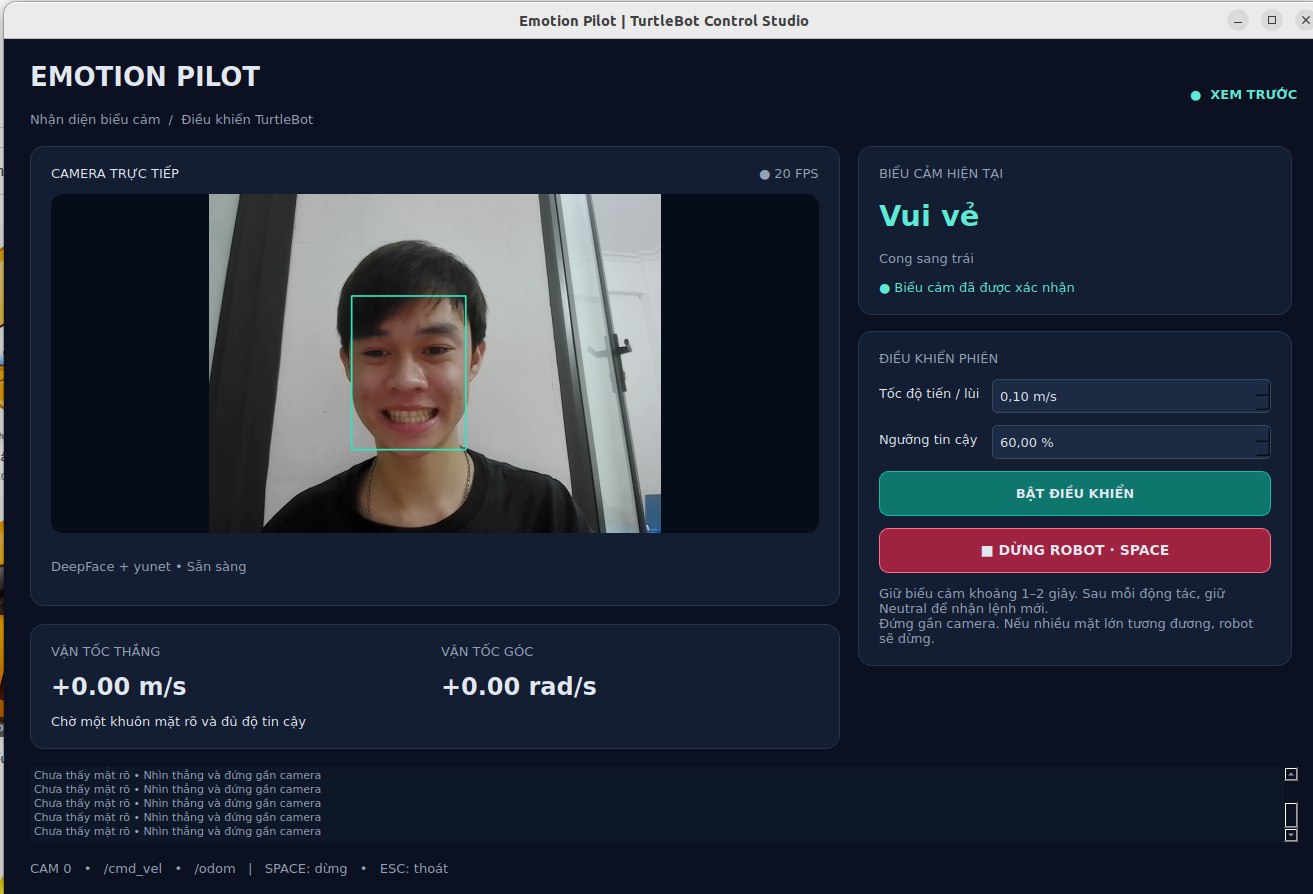
\includegraphics[width=0.96\linewidth]{ketqua/Happy.png}
\caption{Nhận diện Happy: giao diện xác nhận trạng thái Vui vẻ và hành động cong sang trái.}
\label{fig:happy}
\end{figure}

\begin{figure}[H]
\centering
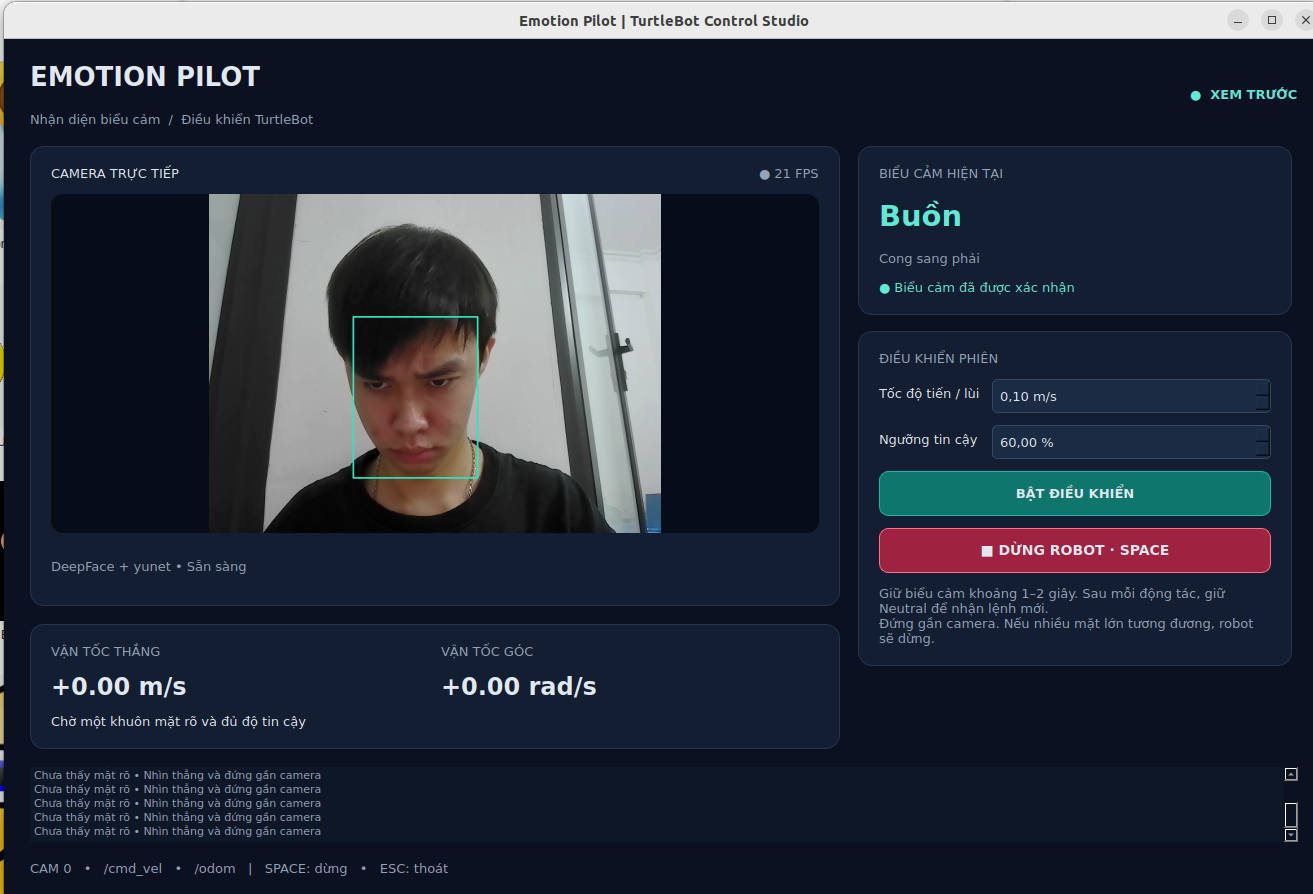
\includegraphics[width=0.96\linewidth]{ketqua/Sad.png}
\caption{Nhận diện Sad: giao diện xác nhận trạng thái Buồn và hành động cong sang phải.}
\label{fig:sad}
\end{figure}

\begin{figure}[H]
\centering
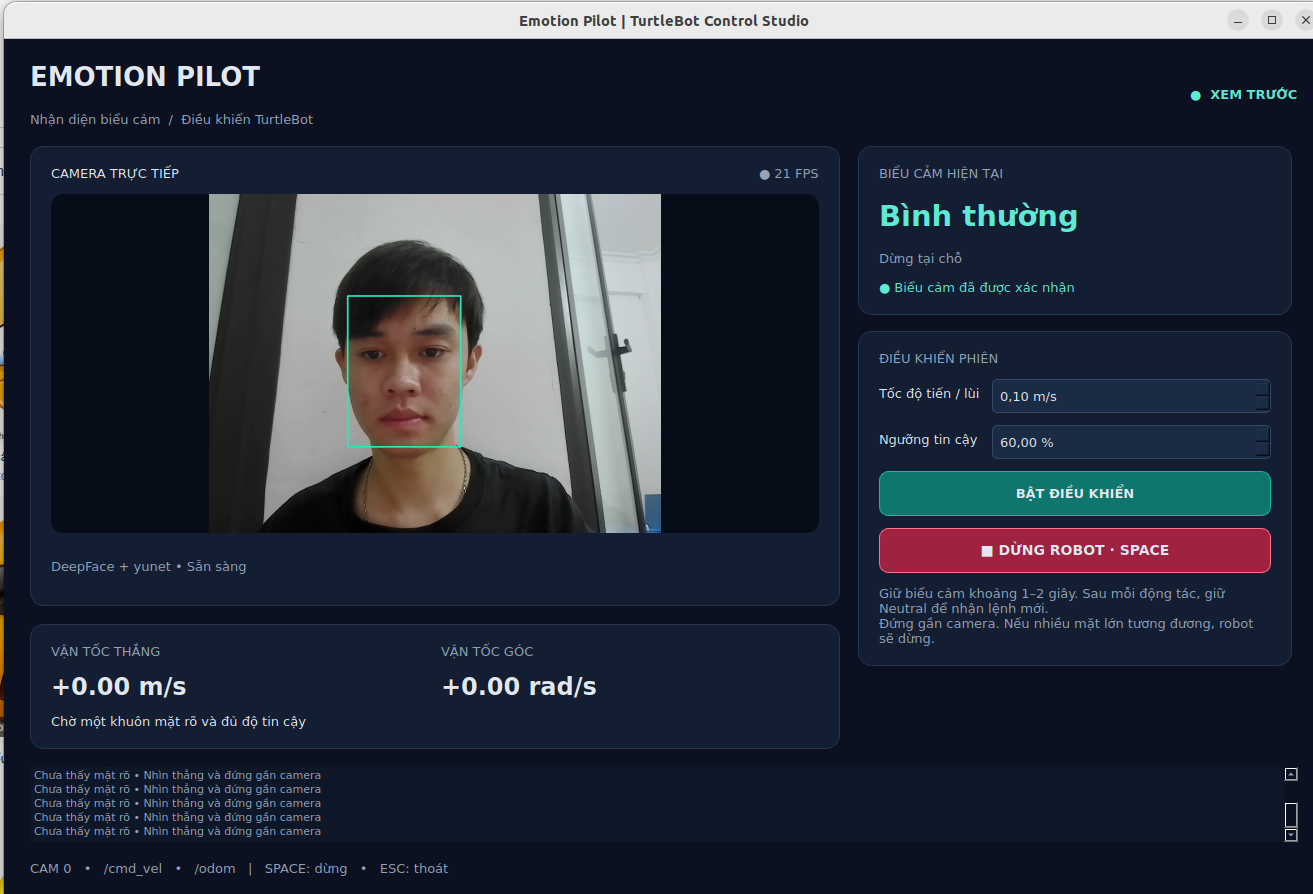
\includegraphics[width=0.96\linewidth]{ketqua/Neutral.png}
\caption{Nhận diện Neutral: giao diện xác nhận trạng thái Bình thường và hành động dừng tại chỗ.}
\label{fig:neutral}
\end{figure}

\begin{figure}[H]
\centering
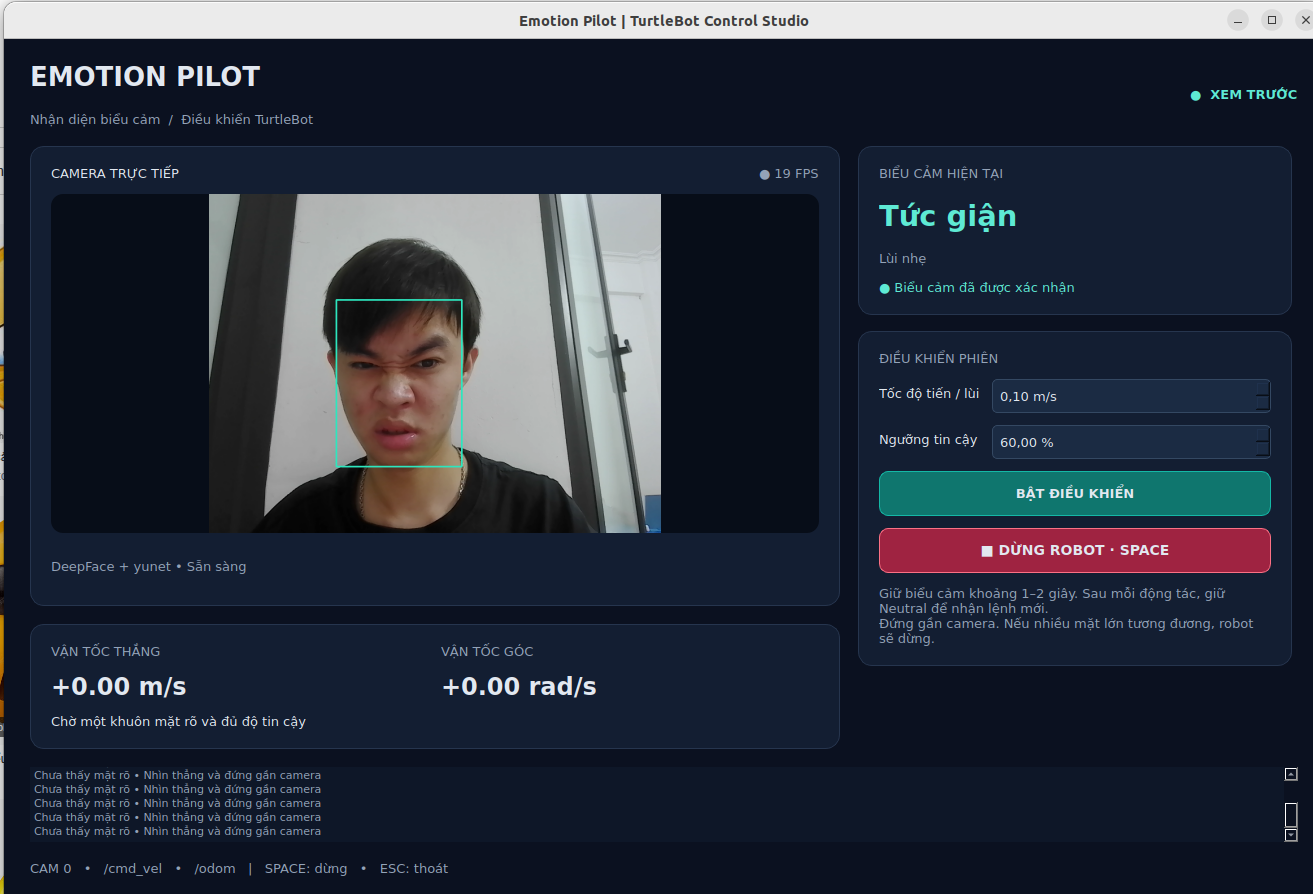
\includegraphics[width=0.96\linewidth]{ketqua/Angry .png}
\caption{Nhận diện Angry: giao diện xác nhận trạng thái Tức giận và hành động lùi.}
\label{fig:angry}
\end{figure}

\begin{figure}[H]
\centering
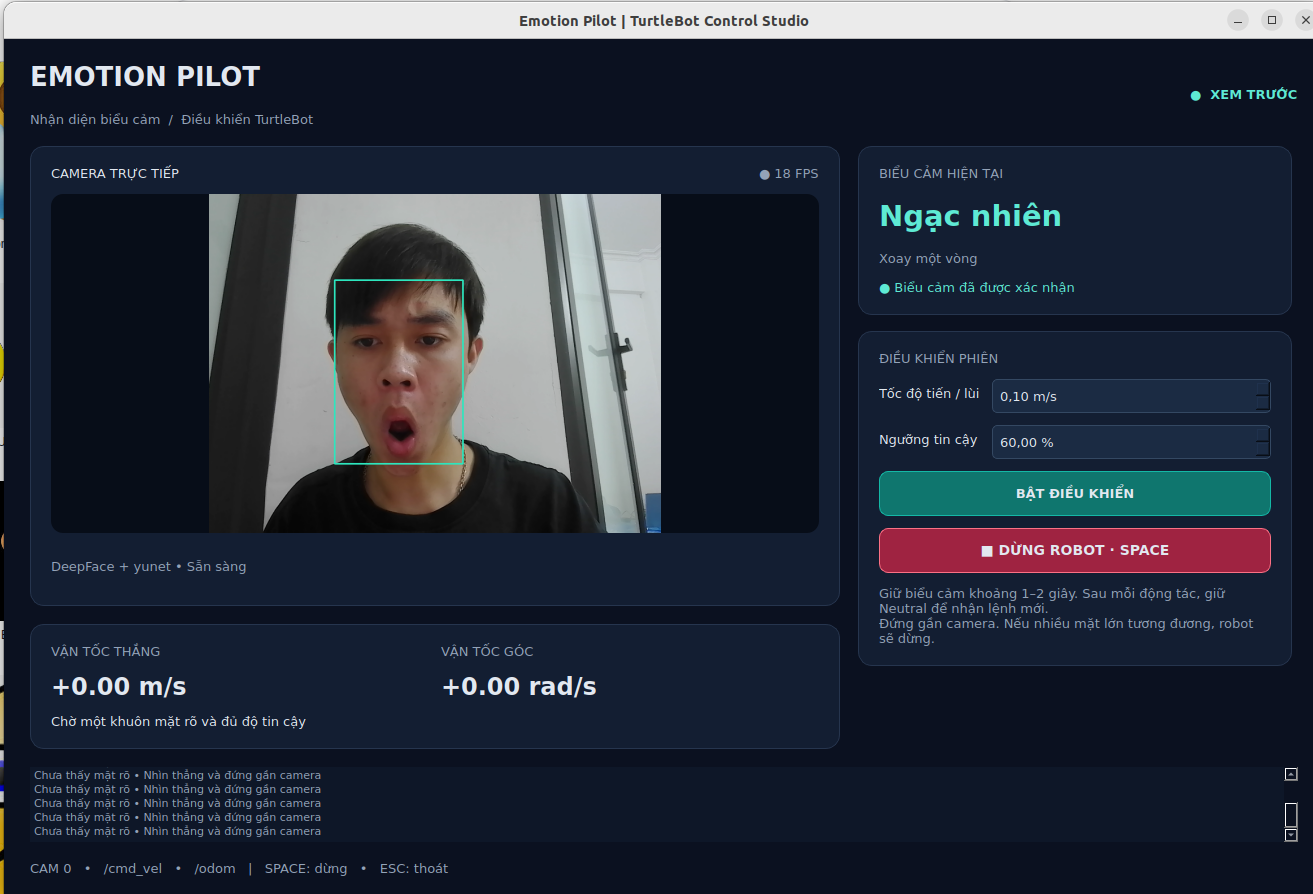
\includegraphics[width=0.96\linewidth]{ketqua/Surprise.png}
\caption{Nhận diện Surprise: giao diện xác nhận trạng thái Ngạc nhiên và hành động xoay một vòng.}
\label{fig:surprise}
\end{figure}

\begin{figure}[H]
\centering
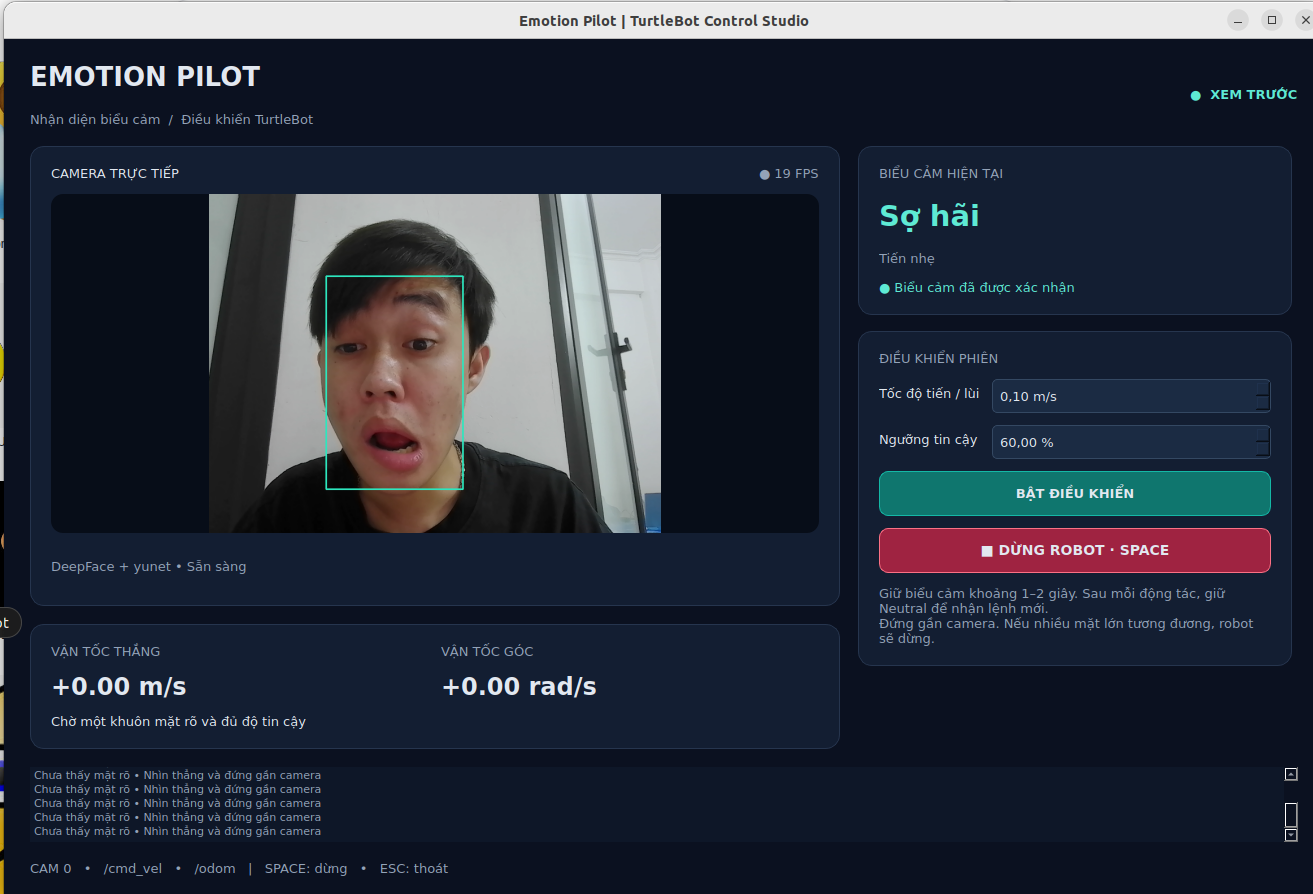
\includegraphics[width=0.96\linewidth]{ketqua/Fear.png}
\caption{Nhận diện Fear: giao diện xác nhận trạng thái Sợ hãi và hành động tiến.}
\label{fig:fear}
\end{figure}

\subsection{Điều khiển trong Gazebo}
Để chạy phần điều khiển, em mở Gazebo qua \code{empty_sim.launch.py}, sau đó mở ứng dụng bằng \cmd{bash run.sh}. Khi mô hình báo sẵn sàng, em bật phiên điều khiển. Khi một biểu cảm đủ điều kiện, bộ điều khiển tạo hành động theo Bảng~\ref{tab:motion}. Trong lúc đang thực hiện, Neutral cho phép dừng và nhận biểu cảm tiếp theo; sau khi hoàn thành tự nhiên, robot chờ Neutral để tránh tự lặp.

Khi quan sát mô phỏng, cần theo dõi cả trạng thái trên giao diện và chuyển động của robot. Riêng các ảnh webcam trong báo cáo chỉ thể hiện kết quả nhận diện. Video demo tại mục cuối báo cáo là nơi bổ sung diễn biến chuyển động liên tục; quãng đường và góc thực tế cần được đối chiếu bằng dữ liệu đo.

\FloatBarrier

\section{Đánh giá kết quả và hướng phát triển}
\subsection{Kết quả đạt được}
\begin{table}[H]
\centering
\renewcommand{\arraystretch}{1.2}
\begin{tabularx}{\linewidth}{@{}L{4.5cm}Y@{}}
\toprule
\textbf{Nội dung} & \textbf{Kết quả} \\
\midrule
Thu hình webcam & Hiển thị được hình ảnh và khung mặt trên giao diện. \\
Khởi tạo mô hình & DeepFace và YuNet báo sẵn sàng trong các ảnh kết quả. \\
Nhận diện sáu trạng thái & Có ảnh xác nhận Happy, Sad, Neutral, Angry, Surprise và Fear. \\
Giao diện & Hiển thị tên biểu cảm, hành động, trạng thái và các nút điều khiển. \\
Tích hợp điều khiển & Đã triển khai phát Twist qua \cmd{/cmd_vel} và nhận \cmd{/odom}. \\
Quỹ đạo đặt & Cung trái/phải $180^\circ$, xoay $360^\circ$, tiến/lùi 1~m danh định. \\
\bottomrule
\end{tabularx}
\caption{Tổng hợp kết quả nhận diện và chức năng đã triển khai.}
\end{table}

Qua các ảnh chụp, em ghi nhận chương trình đã phát hiện được khuôn mặt và xác nhận đủ sáu nhãn trong điều kiện thử của mình. Giao diện hiển thị tên biểu cảm và hành động tương ứng, giúp em theo dõi kết quả mà không cần đọc điểm của từng nhãn.

Chỉ số trên giao diện tại thời điểm chụp nằm trong khoảng 18--21 FPS. Đây là tốc độ cập nhật ảnh hiển thị, không phải tốc độ suy luận của DeepFace. Do ảnh được chọn ở những thời điểm đã xác nhận nhãn, em chưa dùng bộ ảnh này để tính tỷ lệ nhận đúng trên toàn bộ phiên chạy.

Qua phần điều khiển, em thấy cần phân biệt nhãn nhận diện với quyết định phát lệnh. Bộ lọc xử lý kết quả trước khi bộ điều khiển chốt động tác; Neutral và nút dừng giúp người dùng chủ động kết thúc chuyển động. Đây cũng là phần giúp em hiểu rõ hơn cách ghép mô hình nhận diện với một hệ thống điều khiển có trạng thái.

\subsection{Hạn chế của kết quả thực nghiệm}
Chất lượng nhận diện còn phụ thuộc ánh sáng, góc mặt và mức độ rõ của nét mặt. Một số cặp như Happy--Neutral hoặc Fear--Surprise có thể gần nhau khi người dùng thể hiện chưa rõ. Bộ lọc giảm dao động nhưng cũng tạo thêm thời gian chờ trước khi xác nhận.

Cách chọn mặt theo diện tích không theo dõi danh tính. Quãng đường tiến/lùi hiện kết thúc theo thời gian nên có thể lệch so với 1~m danh định. Góc cung tròn và vòng quay được theo dõi bằng odometry, nhưng vẫn chịu ảnh hưởng của chất lượng ước lượng và độ trễ điều khiển. Bài thực hành mới tập trung vào môi trường trống, không xử lý tránh vật cản.

\section{Kết luận}
Trong bài thực hành, em đã xây dựng Emotion Pilot để nhận diện biểu cảm qua webcam bằng DeepFace kết hợp YuNet, hiển thị kết quả bằng PyQt5 và kết nối bộ điều khiển TurtleBot 4 qua ROS 2. Sáu ảnh thực nghiệm cho thấy chương trình có thể xác nhận các nhãn theo yêu cầu trong điều kiện thử của em.

Phần em tập trung hoàn thiện là chọn mặt tiền cảnh, làm ổn định nhãn, chốt động tác và ưu tiên dừng bằng Neutral. Cung nửa vòng và động tác xoay được theo dõi bằng odometry; tiến/lùi sử dụng thời gian theo quãng đường danh định. Qua đó, em hiểu hơn cách chuyển kết quả của một mô hình học sâu thành tín hiệu điều khiển có trạng thái. Hướng tiếp theo là đo nhiều lượt có đối chiếu, cải thiện kết thúc tiến/lùi theo quãng đường và đánh giá trong nhiều điều kiện camera hơn.

\section{Video demo và mã nguồn}
Liên kết mã nguồn và thư mục lưu video demo, tài liệu của bài thực hành:
\begin{itemize}
\item GitHub -- mã nguồn dự án:\\
\url{https://github.com/vanthudat/HRI_Week8}
\item Google Drive -- video demo và tài liệu:\\
\url{https://drive.google.com/drive/folders/MA_THU_MUC}
\end{itemize}

\section*{Tài liệu tham khảo}
\addcontentsline{toc}{section}{Tài liệu tham khảo}
\begin{enumerate}[label={[\arabic*]},leftmargin=2em]
\item \label{ref:deepface} Serengil và cộng sự, \textit{DeepFace}, mã nguồn và hướng dẫn sử dụng phiên bản 0.0.93.\\
\url{https://github.com/serengil/deepface/tree/v0.0.93}
\item \label{ref:twist} ROS 2 Common Interfaces, \textit{geometry\_msgs/msg/Twist}, nhánh Humble.\\
\url{https://github.com/ros2/common_interfaces/blob/humble/geometry_msgs/msg/Twist.msg}
\item \label{ref:odom} ROS 2 Common Interfaces, \textit{nav\_msgs/msg/Odometry}, nhánh Humble.\\
\url{https://github.com/ros2/common_interfaces/blob/humble/nav_msgs/msg/Odometry.msg}
\item \label{ref:gazebo} Open Robotics, \textit{Gazebo Fortress Documentation}.\\
\url{https://gazebosim.org/docs/fortress/}
\item \label{ref:emotionmodel} DeepFace, \textit{Emotion.py}, mã nguồn mô hình phân loại biểu cảm, phiên bản 0.0.93.\\
\url{https://github.com/serengil/deepface/blob/v0.0.93/deepface/models/demography/Emotion.py}
\item \label{ref:yunet} OpenCV, \textit{FaceDetectorYN Class Reference}.\\
\url{https://docs.opencv.org/4.x/df/d20/classcv_1_1FaceDetectorYN.html}
\end{enumerate}

\end{document}


